\documentclass[11pt]{article}
\usepackage[italian]{babel}
\usepackage{geometry}
\usepackage{graphicx}
\geometry{a4paper}
\usepackage{color}
\usepackage{url}
\usepackage[utf8]{inputenc}

\pdfinfo{
   /Author (Alessandro Di Gioacchino)
   /Title  (Specifica del Progetto di Laboratorio - Architettura I - Turno A)
}

\title{Specifica del Progetto di Laboratorio \\ Architettura degli Elaboratori I}

\author{Alessandro Di Gioacchino\\ Matricola: 931271, Turno: A\\ \url{alessandro.digioacchino@studenti.unimi.it}}

\date{}


\begin{document}

\maketitle

In questo progetto è proposta una possibile implementazione del gioco da me battezzato {\itshape Spegni le luci}. 

Sia il sistema di input che quello di output sono costituiti da una scacchiera di dimensioni 3$\times$3: il primo è composto da bottoni, il secondo da LED; è inoltre presente un tasto per accendere o spegnere il gioco. Alla pressione di tale tasto, una serie di generatori di numeri random provvede ad illuminare alcune delle luci in un pattern pseudo-casuale. Scopo dell'utente è quello di spegnerle tutte, prestando attenzione al fatto che la pressione di un bottone non causerà unicamente lo spegnimento (o accensione) della luce corrispondente, ma anche di quelle ad essa adiacenti.

\begin{figure}[!htpb]
\centering
\includegraphics[width=0.8\columnwidth]{Immagini/"Spegni le luci"}
\caption{\footnotesize{Il sistema di input e di output {\itshape (versione provvisoria)}. Alla pressione del tasto On / off, le luci numero 1, 3, 5, 7, 8 sono state accese in maniera pseudo-random; l'utente ha successivamente premuto il tasto 8, causando lo spegnimento delle luci 5, 7, 8 e l'accensione della luce 9; dopodiché ha premuto il tasto 6, accendendo le luci 5, 6 e spegnendo le luci 3, 9; infine, premendo il tasto 2, ha spento le luci 1, 5 e acceso le luci 2, 3. A questo punto, l'utente ha la possibilità di vincere attraverso il tasto 3.}}
\label{fig:spegnileluci}
\end{figure}

Per memorizzare lo stato dei LED sono necessari degli elementi di memoria asincroni, uno per LED; deve anche essere possibile impostare a zero il loro contenuto, in modo da simulare lo spegnimento del gioco alla pressione dell'apposito pulsante.

\begin{figure}[!htpb]
\centering
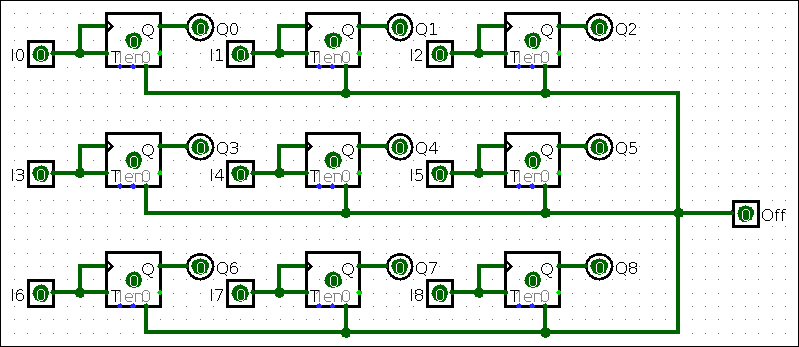
\includegraphics[width=0.8\columnwidth]{Immagini/Display}
\caption{\footnotesize{Flip-flop per memorizzare lo stato dell'output {\itshape (versione provvisoria)}. Il dato in input a tali elementi di memoria è collegato anche all'ingresso del clock, rendendoli di fatto asincroni. L'immagine mostra in che modo l'output dei flip-flop varia in base all'interazione dell'utente con il circuito.
\textbf {N.B. La Figura 1 e la Figura 2 sono state catturate durante partite distinte.}}}
\label{fig:display}
\end{figure}

Anche i generatori di numeri random sono asincroni, e cambiano il loro stato solamente quando il giocatore preme il tasto di accensione: in questo modo si può ottenere l'effetto descritto inizialmente, cioè l'accensione dei LED in maniera semi-randomica.

\begin{figure}[!htpb]
\centering
\includegraphics[width=0.6\columnwidth]{Immagini/"Inizio casuale"}
\caption{\footnotesize{Generatori di numeri casuali da un bit {\itshape (versione provvisoria)}. L'uscita di ciascun generatore è posta in AND con il segnale del tasto On / off: in questo modo, dopo aver acceso alcune luci il circuito può restituire il controllo all'utente, il quale ottiene così l'esclusività sul sistema di input. Nel caso in cui nessuna delle luci sia illuminata, il circuito provvederà ad indicarlo all'utente mediante il segnale di Errore.}}
\label{fig:iniziocasuale}
\end{figure}

Il circuito che gestisce l'input è costituito da una serie di porte logiche OR, il cui scopo è quello di innescare il cambio di stato degli elementi di memoria che gestiscono il display in modo da simularne la propagazione. In altri termini, non c'è una corrispondenza biunivoca tra il sistema di input e quello di output, poiché un unico bottone controlla due o più LED.
\end{document}